An organization which needs to host multiple services like e-mail servers,
web servers, file downloading servers, e-commerce websites, etc may either opt
to own, maintain and manage their own 
infrastructure (i.e., private\index{Private cloud} 
clouds~\cite{ubuntu-private-cloud}), 
or alternatively, use the services provided by public hosting 
centers (i.e., public\index{Public cloud} clouds~\cite{ec2}). 
In traditional datacenters (before virtualization), multiple
servers would run as separate processes on the same machine and such
mapping would exist from subsets of processes to a set of physical machines.
Guaranteeing resource isolation could be possible only by hosting a single
server on a single physical machine, but would 
cause resource under-utilization
during periods of light loads.

For instance, an auction website may have
periods of heavy load during the day and be comparatively lightly-loaded
during the night. Hence, it may be profitable to the hosting center provider to
host multiple auction websites on the same machine during the night while
assigning them separate machines during the day. However, such adjustments
would need manual intervention or tedious automation to plan/set them up.
Typically, tedious automation and/or manual intervention to provision 
resources based on workload levels, would be well avoided and traditional
hosting centers would just provision the servers for peak load.
However, such static allocation of resources to each server is wasteful
and inefficient because
the server is not expected to be handling peak load at all 
times~\cite{capacity-planning, emerging-research-directions}. Also, with
such static allocation, initial deployment of a server in the data-center
will involve procurement and setup delays of the physical 
machines\index{Physical machine}~\cite{xen-art-of-virtualization}. 

Virtualization\index{Virtualization} helps to avoid
such pitfalls, by enabling dynamic resource allocation and 
quicker deployment
of services. Instead of installing new hardware for deploying/scaling a server
in the data-center, virtualization 
allows transparent, on-demand deployment on a few
processors in an existing multi-processor machine and avoids new machine
procurement delays~\cite{xen-art-of-virtualization}. 
Virtualization allows accomodation of varying load-levels by
on-demand resource allocation~\cite{xen-art-of-virtualization-revisited}
and also helps reduce application downtime~\cite{google-live-migration}. 
Due to above benefits of virtualization, 
many hosting centers have moved from providing Hardware as a 
Service (HaaS)\nomenclature{HaaS:}{Hardware as a Service}\index{HaaS}
to Infrastructure as a 
Service (IaaS)\nomenclature{IaaS:}{Infrastructure as a 
Service}\index{IaaS} instead~\cite{ec2, azure}. 
The primary difference between HaaS and IaaS is that the 
former involves use or leasing of physical
hardware/machine whereas the latter involves 
leasing of virtual resources/machines\index{Virtual machine}.


\subsection{Virtualization}
Virtualization is a technology that allows abstraction of network, storage
and compute services, by providing a software middle-layer between the
physical hardware and the applications that run on it.
Hence, each physical machine (PM)\index{PM} 
can host multiple virtual machines (VMs)\index{VM},
such that each virtual machine sees an
abstraction of resources on which it executes. This makes it easy
to start, stop, move or increase the number of virtual machines hosted
on one or more physical machines.

To motivate the use of virtualization, let us consider a similar example.
Suppose an organization needs to host fifty software 
applications\textemdash{}webservers, email servers, file servers and so on.
Based on some back-of-the-envelope calculation of resource requirements,
suppose twenty physical machines are procured for this purpose.
In the absence of virtualization, a subset of servers each, would be hosted
on each physical machine and each might be typically
peak-provisioned~\cite{berkeley-view}. 
The selection of which subset of servers can/should
be hosted together on a single machine may be random or may depend on
considerations like
OS platform issues, licensing issues, hardware capacity, software/hardware
version compatibilities, etc. Some subset of servers may even be grouped
together if they have mutually exclusive resource requirements (say
CPU-bound webservers and 
IO-bound database servers 
hosted together~\cite{dynamic-provisioning-multi-tier}) 
because there is a perceived high-level guarantee that neither 
one will encroach on the resource
requirements of the other, 
thus providing approximate resource isolation.
However, resource isolation guarantees can be provided only with kernel 
changes and/or real-time operating systems~\cite{enforcing-isolation}.

A user who invests in hosting services would prefer to get hard guarantees
on resource and performance isolation instead of being subject
to the vagaries of resource utilization of other colocated processes
or applications. 
Moreover, in case of \textit{public clouds}, 
the user would also prefer to be paying only for
utilized resources and not for unused resources~\cite{berkeley-view}. This is
where virtualization offers a good solution. A virtual machine gives
an entire machine-like resource environment with usability of any
operating system. And thus, the user need only be charged for the resources
being allocated to their virtual machine~\cite{ec2}.

Virtualization allows each server process to be provided with its own
resource environment and guarantees a fixed amount of resources such that
its resource availability and performance levels will not be affected by
any other colocated process's resource usage.
Such guarantees are possible owing to the
virtualization middle-layer, or the 
Virtual Machine Monitor (VMM)\index{VMM}, which
arbitrates communication back-and-forth between the applications and the
hardware. Basically, each application gets
its own (virtualized) environment, 
known as a \textit{Virtual Container} or a
\textit{Virtual Machine} and it may be even unaware that 
its container is not a
physical machine with access to real hardware i.e. virtualization is
transparent to the applications/services themselves. Each virtual machine
runs like a separate operating-system instance and has interfaces for
direct or indirect access to the physical hardware. The OS\footnote{OS stands
for Operating System} executing within the virtual machine is referred to
as a \textit{guest OS}\index{Guest OS} while the original 
operating system on the physical
machine which provides the virtualization support is referred to as
the \textit{host OS}\index{Host OS}.

Example instantiations of
virtualization-based solutions are, (i) users/clients hosting their
applications on a remote dataCenter\index{Datacenter} 
and negotiating for service level agreements\index{SLA}
%(henceforth referred to as a \textit{Public Cloud}).
and (ii) enterprises hosting applications and services on a
private self-managed cluster of machines, for internal and external
access.
%(henceforth referred to as a \textit{Private Cloud}).
In the latter
example, both the user and the provider may be one and the same.
Virtualization offers benefits to both users and providers 
of the datacenter.
Traditionally, an end user would be burdened with planning, acquiring
and deployment of infrastructure, 
and also regular maintenance~\cite{berkeley-view}. The end-user
would require to plan software updates and hardware upgrades as the system
grows, and also manage low-level decisions to maintain performance
requirements. However, with virtualization, the end user is responsible only
to pay for the resources on-demand, while receiving guarantees on performance.
The end-user can be agnostic of physical hardware issues. At the back-end,
the service provider benefits by way of potential opportunities to
effectively multiplex available resources~\cite{vm-multiplexing}, 
provide on-demand \& scalable service~\cite{google-live-migration} 
that is centrally managed, and cut down on expenses.

\begin{figure}[t]
\begin{center}
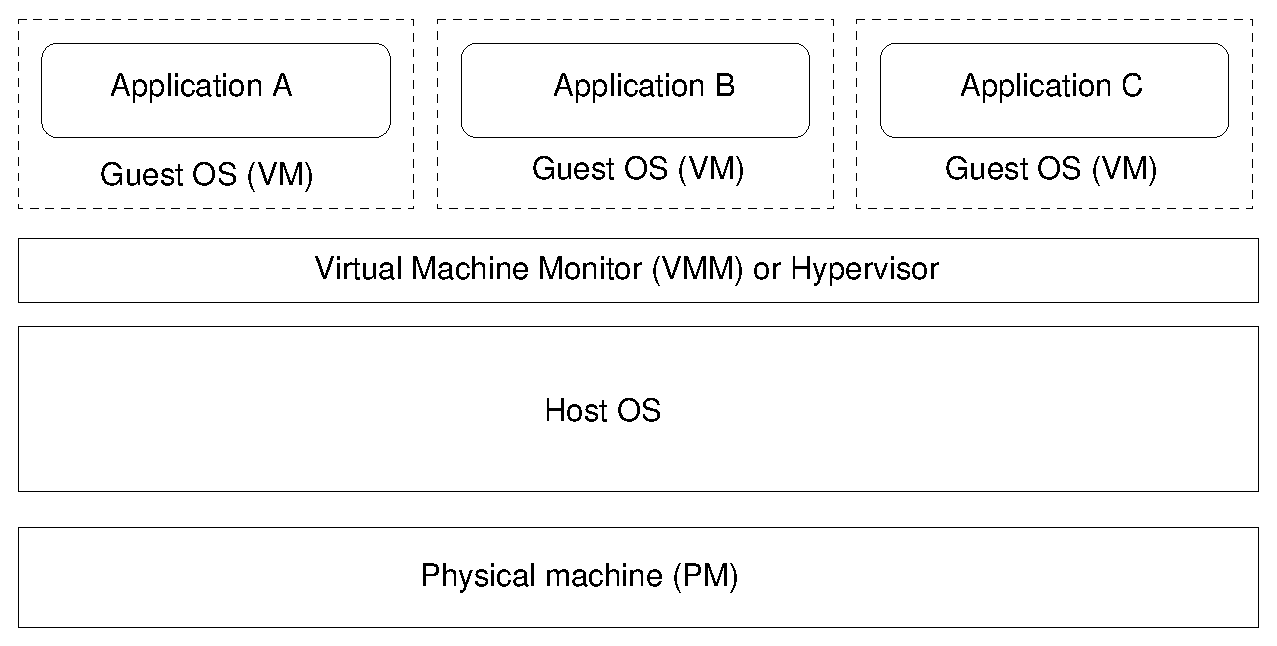
\includegraphics[height=7cm, width=14cm]{first-aps-figures/virtualization-arch.eps}
\caption{Virtualization framework architecture: \textit{A physical machine is 
virtualized using a VMM such that it is capable of hosting multiple virtual 
machines that have their own operating systems (OS) each. The VMM is thus, a
middleware that handles and delegates the responsibilities related to virtualization
of the physical machine.}} 
\label{virtualization-arch}
\end{center}
\end{figure}

\subsection{Virtualization techniques}
\label{virtualization-tech}
There are various virtualization techniques: \textit{full-virtualization}~\cite{vmware-paravirtualization},
\textit{para-virtualization}~\cite{xen}, \textit{OS-level
virtualization}~\cite{quantifying-the-performance-isolation-properties}
and \textit{hardware-assisted virtualization}~\cite{kvm}.
Fig.~\ref{virtualization-arch} shows the basic architecture of the
virtualization framework. As seen in the figure, a host operating
system, instrumented with the 
Virtual Machine Monitor (VMM)\index{VMM} or Hypervisor\index{Hypervisor},
executes on the physical machine, 
and one or more VMs, containing guest operating systems, execute on top 
of the virtualization layer.


\underline{Full-virtualization}\index{Full-virtualization}: In 
this technique, the guest 
OS can run unmodified within the virtual machine. This is made 
possible by the use of Binary translation and
Direct execution techniques~\cite{vmware-paravirtualization}. 
\textit{Binary translation} refers to the ``on-the-fly substitution'' 
of traditional guest OS instructions with a virtual sequence of 
instructions and, \textit{Direct execution}
strategy is adopted for executing user-level code. So the
guest OS is completely decoupled from the underlying hardware by the
virtualization layer.
Binary translation is used in VMware's full-virtualization 
solution~\cite{vmware-paravirtualization} due to challenges
in virtualizing privileged operations, like I/O instructions. This is
because if a guest OS is directly allowed to execute the privileged I/O
instructions, it could alter the
state of other guest OSes and compromise security. 

\underline{Para-virtualization}\index{Para-virtualization} tries 
to address the concern of
I/O virtualization another way, by making changes to the guest
OS such that privileged I/O instructions cause traps to the hypervisor and are
executed by it on behalf of the guest OS. For example, request for an I/O
operation by the guest OS will
be made in the form of a function call that does not actually perform
the I/O operation, but merely requests the hypervisor to perform it.
The hypervisor will execute the I/O after checking for requisite permissions,
and will intimate the guest OS when task is over.

\underline{OS-assisted virtualization}\index{OS-assisted virtualization}: 
In this technique, guest operating systems\index{Guest OS} are processes 
that are allocated different namespaces such that
they seem to be separate machines altogether. However, in OS-level
virtualization, the same host OS\index{Host OS} kernel also supports 
the guest processes.
The advantage of full-virtualization and paravirtualization over OS-level
virtualization is that they can support heterogeneous operating system
distributions as guest OSes, like Linux, BSD and Windows
XP~\cite{xen-art-of-virtualization}. 
Although paravirtualization is also an OS-assisted form of virtualization 
requiring all privileged instructions to be executed by the virtualization
layer, the difference is that para-virtualization can support
different guest operating systems whereas OS-level virtualization cannot.

\underline{Hardware-assisted virtualization}\index{Hardware-assisted virtualization}: 
In this technique,
the hardware is enhanced with virtualization awareness such that
the CPU itself traps the privileged/sensitive instructions and emulates
the instructions in hardware instead of software, hence obviating the need
for binary translation or paravirtualization. Hardware-assisted virtualization
is also a form of full virtualization since the guest OS can remain ignorant
of the virtualization involved~\cite{hardware-assisted-wiki}.
% However, hardware assisted virtualization technique
% is still in its infancy and has not become much popular yet.

Based on the above
types, there are several virtualization technologies
like Xen~\cite{xen-art-of-virtualization}\index{Xen},
Vmware~\cite{vmware-paravirtualization}\index{Vmware},
KVM~\cite{kvm}\index{KVM} and OpenVZ~\cite{OpenVZ}\index{OpenVZ}. 
Xen is an
example of para-virtualization, KVM and VMware are examples of
full-virtualization and OpenVZ is an example of OS-level
virtualization.
